\documentclass[tikz, border=7pt]{standalone}
\usepackage{tikz}
\usepackage{tkz-euclide}
\usepackage{amsmath}
\usepackage{amsfonts}
\usepackage{amssymb}


\newcommand\Mydiv[2]{%
$\strut#1$\kern.25em\smash{\raise.3ex\hbox{$\big)$}}$\mkern-8mu
        \overline{\enspace\strut#2}$}
\begin{document}
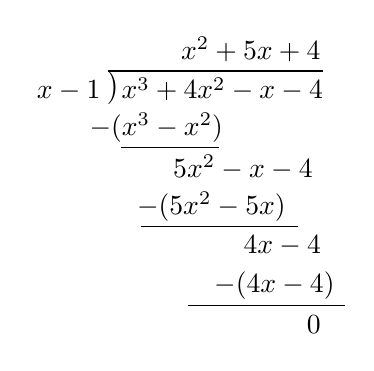
\begin{tikzpicture}

\node (c) at (0.5,3) {\Mydiv{x-1}{x^3+4x^2-x-4}};
\node (c) at (0.2,2.5) {$-(x^3-x^2)$};
\draw (-0.25, 2.25) -- (1,2.25);
\node (c) at (1.3,2) {$5x^2-x-4$};
\node (c) at (0.9,1.5) {$-(5x^2-5x)$};
\draw (0, 1.25) -- (2,1.25);
\node (c) at (1.8,1) {$4x-4$};
\node (c) at (1.7,0.5) {$-(4x-4)$};
\draw (0.6, .25) -- (2.6,.25);
\node (c) at (2.2,0) {$0$};

\node (c) at (1.4,3.5) {$x^2+5x+4$};



\end{tikzpicture}
\end{document}
